\subsection{Dependency viewpoint}

    \subsubsection{UML dependency diagram}
        \begin{figure}[!ht]
            \centering
            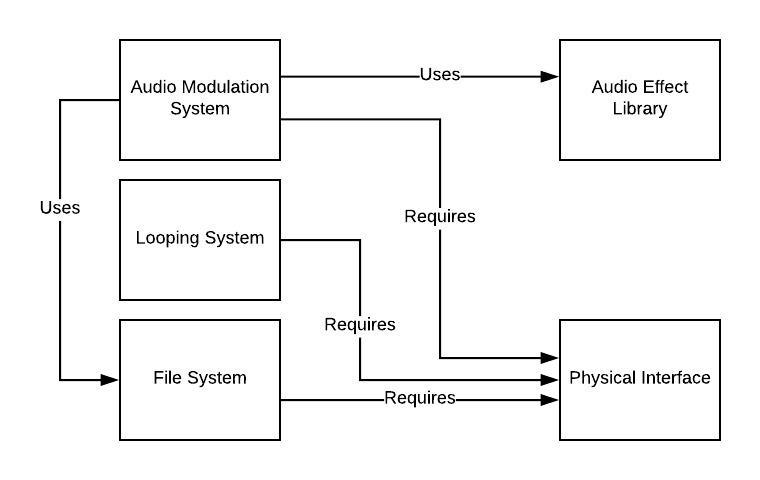
\includegraphics{diagrams/dependency-diagram.jpeg}
            \caption{Dependency diagram}
            \label{fig:dependency}
        \end{figure}
    \subsubsection{Dependencies attribute}
       Figure \ref{fig:dependency} shows the development dependencies for each subsystem. The first subsystems that can be designed are the Audio Modulation and Looping subsystems. The Looping subsystem design independent from other components and can be developed at any time before the Physical Interface. The design of the Audio Modulation Subsystem is used to inform the Audio Effect Library and the File System designs. Once the software subsystems (Audio Modulation System, Looping System, and File System) are designed, work can begin on the Physical Interface design to create an interface that will adequately and efficiently control all three software subsystems.
        